\documentclass[12pt]{article}

\usepackage{amsmath}
\usepackage{amsfonts}
\usepackage{amssymb}
\usepackage{graphicx}

\title{Circle Cuts (Draft)}

\begin{document}

\maketitle

Starting from a circle, the first cut must be made vertically down the center.

\begin{figure}[h]
    \centering
    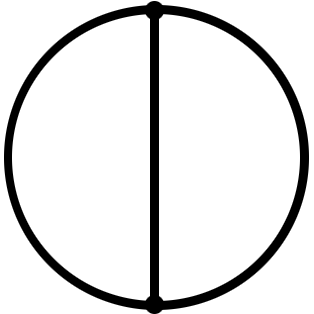
\includegraphics[width=0.10\textwidth]{cut1.png}
    \label{fig:first_cut}
\end{figure}

The resulting figure is comprised of two shapes, both half circles with one strait face
and one arc segment. Then, from this state or any future state, you may cut one shape inside
the figure between its edges under the following restrictions:

\begin{enumerate}
    \item When making a new cut, its ends must be equidistant from the ends of adjacent cuts on the same edge.
    \item A cut must create two shapes with non-zero area.
\end{enumerate}

After the second cut, the figure may be in one of the following four configurations:

\begin{figure}[h]
    \centering
    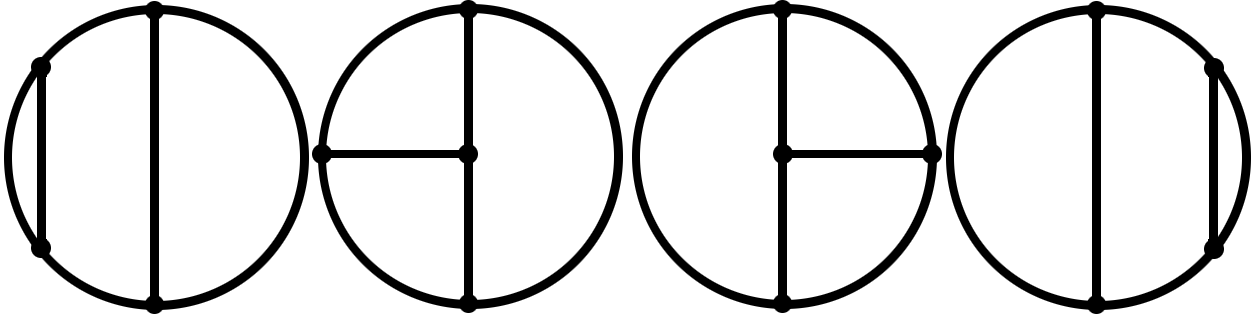
\includegraphics[width=0.40\textwidth]{cut2.png}
    \label{fig:first_cut}
\end{figure}

How many distinct configurations are possible after $n$ cuts?

\end{document}
